\documentclass[11pt,letterpaper]{article}
\usepackage[sinindice]{tecnm}
\usepackage{tikz}
\usetikzlibrary{arrows.meta,positioning,shapes.geometric,trees}
\usepackage{booktabs,array,amsmath,amssymb,multirow}
\usepackage{float}     % Permite el uso de [H] para fijar la posición de flotantes
\usepackage{tabularx}  % Tablas ajustadas a la anchura del texto (\linewidth)

\materia{Inteligencia Artificial y su Ética}
\actividad{Tema 2.2 - Actividad 9 \\ Algoritmos de Búsqueda sin Información}
\profesor{M. Lilia Ureña Lugo}

% Estilos de nodos para diagramas TikZ
\tikzset{
  inicio/.style={draw=blue!70!black,fill=blue!15,rounded corners=3pt,thick,align=center,font=\tiny,inner sep=2pt,minimum width=1.3cm},
  meta/.style={draw=green!50!black,fill=green!25,rounded corners=3pt,thick,align=center,font=\tiny,inner sep=2pt,minimum width=1.3cm},
  visitado/.style={draw=orange!80!black,fill=orange!20,rounded corners=3pt,thick,align=center,font=\tiny,inner sep=2pt,minimum width=1.3cm},
  novisitado/.style={draw=gray!50,fill=gray!10,rounded corners=3pt,dashed,align=center,font=\tiny,inner sep=2pt,minimum width=1.3cm}
}

\begin{document}
\portada
\indicegeneral

\section{Introducción}

Los algoritmos de búsqueda sin información exploran el espacio de estados sin utilizar conocimiento previo sobre el costo restante hacia la meta \parencite{iae_u2_diseno}. En esta actividad se analizan y diferencian visualmente las dos estrategias fundamentales las cuales son la Búsqueda en Anchura (BFS, siglas en inglés de \textit{Breadth-First Search}) y Búsqueda en Profundidad (DFS, siglas en inglés de \textit{Depth-First Search}).

\begin{itemize}
  \item \textbf{BFS:} Utiliza una estructura de cola (FIFO). Expande el espacio de estados nivel por nivel antes de pasar al siguiente nivel de profundidad \parencite{iae_u2_diseno}.
  \item \textbf{DFS:} Utiliza una estructura de pila (LIFO). Explora una rama en su máxima profundidad posible antes de realizar \textit{backtracking} y evaluar ramas alternativas \parencite{iae_u2_diseno}.
\end{itemize}

%% ===================== EJERCICIO 1 =====================
\section{Ejercicio 1: Las jarras de agua (4L y 3L)}

\subsection{Representación Formal}
\begin{itemize}
  \item \textbf{Estado:} Par ordenado $(x,y) \in \{0,1,2,3,4\} \times \{0,1,2,3\}$.
  \item \textbf{Estado inicial:} $s_0 = (0,0)$.
  \item \textbf{Estado meta:} $G = \{(2,y) \mid 0 \le y \le 3\}$.
\end{itemize}

\subsection{Árboles de Búsqueda y Orden de Exploración (BFS vs. DFS)}

En la Figura~\ref{fig:jarras_bfs_dfs} se contrasta el recorrido en anchura frente al recorrido en profundidad, disponiendo ambos árboles lado a lado e indicando en cada nodo el orden numérico de visita ($[1], [2], \dots$).

\begin{figure}[H]
\centering
% Columna Izquierda: BFS
\begin{minipage}[t]{0.48\linewidth}
\centering
\textbf{\scriptsize a) Recorrido por Anchura (BFS)}\\[4pt]
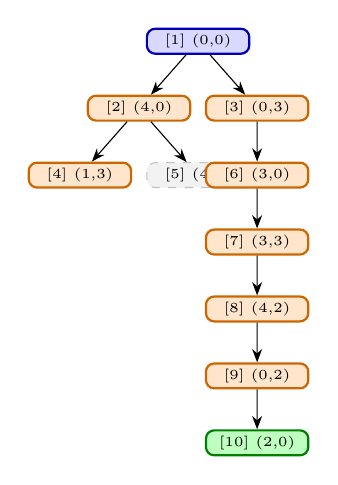
\begin{tikzpicture}[level distance=0.85cm, sibling distance=1.5cm, ->, >=Stealth]
\node[inicio] (r) {[1] (0,0)}
  child {node[visitado] {[2] (4,0)}
    child {node[visitado] {[4] (1,3)}}
    child {node[novisitado] {[5] (4,3)}}
  }
  child {node[visitado] {[3] (0,3)}
    child {node[visitado] {[6] (3,0)}
      child {node[visitado] {[7] (3,3)}
        child {node[visitado] {[8] (4,2)}
          child {node[visitado] {[9] (0,2)}
            child {node[meta] {[10] (2,0)}}
          }
        }
      }
    }
  };
\end{tikzpicture}
\end{minipage}
\hfill
% Columna Derecha: DFS
\begin{minipage}[t]{0.48\linewidth}
\centering
\textbf{\scriptsize b) Recorrido por Profundidad (DFS)}\\[4pt]
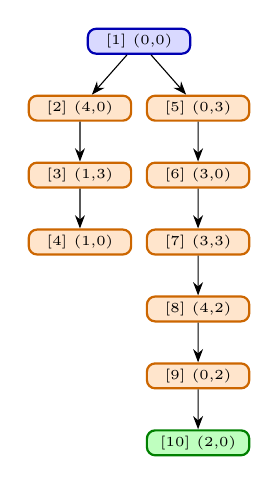
\begin{tikzpicture}[level distance=0.85cm, sibling distance=1.5cm, ->, >=Stealth]
\node[inicio] (r) {[1] (0,0)}
  child {node[visitado] {[2] (4,0)}
    child {node[visitado] {[3] (1,3)}
      child {node[visitado] {[4] (1,0)}}
    }
  }
  child {node[visitado] {[5] (0,3)}
    child {node[visitado] {[6] (3,0)}
      child {node[visitado] {[7] (3,3)}
        child {node[visitado] {[8] (4,2)}
          child {node[visitado] {[9] (0,2)}
            child {node[meta] {[10] (2,0)}}
          }
        }
      }
    }
  };
\end{tikzpicture}
\end{minipage}
\caption{Comparación de los recorridos BFS y DFS para el Ejercicio 1.}
\label{fig:jarras_bfs_dfs}
\end{figure}

Al observar la Figura~\ref{fig:jarras_bfs_dfs}, se aprecia cómo opera cada estrategia: en \textbf{BFS (a)}, el algoritmo expande el espacio de estados de forma horizontal, evaluando los nodos inmediatos $[2]$ y $[3]$ en el Nivel 1 antes de profundizar al Nivel 2. Por su parte, en \textbf{DFS (b)} el algoritmo se adentra de forma vertical en la rama izquierda (nodos $[2] \to [3] \to [4]$); al agotar las transiciones de esa línea sin hallar la meta, realiza \textit{backtracking} hasta la raíz $[1]$ para descender por la rama derecha ($[5]$ a $[10]$) hasta alcanzar la solución en el estado meta $(2,0)$.

\subsection{Análisis Comparativo del Ejercicio 1}

\begin{table}[H]
\centering\small
\renewcommand{\arraystretch}{1.2}
\begin{tabularx}{\linewidth}{@{} l X X @{}}
\toprule
\textbf{Criterio de Evaluación} & \textbf{Búsqueda en Anchura (BFS)} & \textbf{Búsqueda en Profundidad (DFS)} \\
\midrule
\textbf{Estructura de Datos} & Cola / FIFO & Pila / LIFO \\
\textbf{Nodos Generados} & 14 nodos en total & 14 nodos en total \\
\textbf{Nodos Explorados} & 10 nodos (evalúa el nivel completo) & 10 nodos (profundiza en ramas activas) \\
\textbf{Profundidad de Solución ($d$)} & $d = 6$ pasos & $d = 6$ pasos \\
% \textbf{Uso de Memoria} & $O(b^d)$ — Almacena todos los nodos del nivel & $O(b \cdot m)$ — Guarda únicamente el camino actual \\
\textbf{Completitud} & Completo (encuentra la solución en grafos finitos) & Completo (con control de ciclos) \\
\textbf{Optimalidad} & Óptimo (garantiza el mínimo de pasos) & No óptimo (puede seguir ramas subóptimas) \\
\bottomrule
\end{tabularx}
\caption{Análisis de los parámetros de rendimiento para el Ejercicio 1.}
\end{table}

%% ===================== EJERCICIO 2 =====================
\section{Ejercicio 2: El pastor, el lobo, la cabra y la lechuga}

\subsection{Representación Formal}
\begin{itemize}
  \item \textbf{Estado:} Tupla $(p, l, c, h) \in \{0,1\}^4$ ($0=\text{Orilla A}, 1=\text{Orilla B}$).
  \item \textbf{Estado inicial:} $s_0 = (0,0,0,0)$.
  \item \textbf{Estado meta:} $G = \{(1,1,1,1)\}$.
\end{itemize}

\subsection{Árboles de Búsqueda BFS vs. DFS}

\begin{figure}[H]
\centering
\begin{minipage}[t]{0.48\linewidth}
\centering
\textbf{\scriptsize a) Recorrido por Anchura (BFS)}\\[4pt]
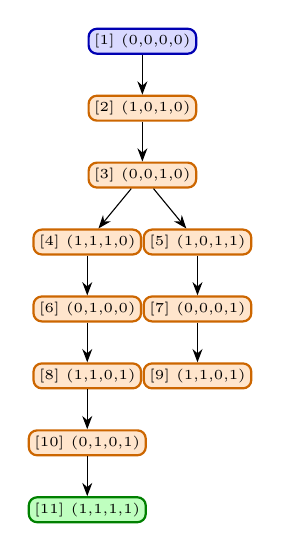
\begin{tikzpicture}[level distance=0.85cm, sibling distance=1.4cm, ->, >=Stealth]
\node[inicio] {[1] (0,0,0,0)}
  child {node[visitado] {[2] (1,0,1,0)}
    child {node[visitado] {[3] (0,0,1,0)}
      child {node[visitado] {[4] (1,1,1,0)}
        child {node[visitado] {[6] (0,1,0,0)}
          child {node[visitado] {[8] (1,1,0,1)}
            child {node[visitado] {[10] (0,1,0,1)}
              child {node[meta] {[11] (1,1,1,1)}}
            }
          }
        }
      }
      child {node[visitado] {[5] (1,0,1,1)}
        child {node[visitado] {[7] (0,0,0,1)}
          child {node[visitado] {[9] (1,1,0,1)}}
        }
      }
    }
  };
\end{tikzpicture}
\end{minipage}
\hfill
\begin{minipage}[t]{0.48\linewidth}
\centering
\textbf{\scriptsize b) Recorrido por Profundidad (DFS)}\\[4pt]
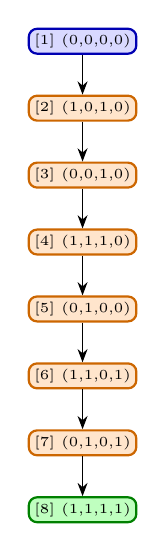
\begin{tikzpicture}[level distance=0.85cm, sibling distance=1.4cm, ->, >=Stealth]
\node[inicio] {[1] (0,0,0,0)}
  child {node[visitado] {[2] (1,0,1,0)}
    child {node[visitado] {[3] (0,0,1,0)}
      child {node[visitado] {[4] (1,1,1,0)}
        child {node[visitado] {[5] (0,1,0,0)}
          child {node[visitado] {[6] (1,1,0,1)}
            child {node[visitado] {[7] (0,1,0,1)}
              child {node[meta] {[8] (1,1,1,1)}}
            }
          }
        }
      }
    }
  };
\end{tikzpicture}
\end{minipage}
\caption{Diferenciación gráfica de los recorridos BFS y DFS para el Ejercicio 2.}
\label{fig:pastor_bfs_dfs}
\end{figure}

En la Figura~\ref{fig:pastor_bfs_dfs} se contrapone el comportamiento de ambos métodos en el cruce del río: \textbf{BFS (a)} evalúa simultáneamente las dos alternativas seguras surgidas tras regresar la cabra ($[4]$ cruzando con el lobo y $[5]$ cruzando con la lechuga), lo que implica mantener más nodos abiertos en la memoria. En cambio, \textbf{DFS (b)} selecciona la primera alternativa válida ($[4]$ con el lobo) y avanza verticalmente sin desviarse por la otra rama, alcanzando la meta en el paso $[8]$ con un número menor de nodos explorados.

\subsection{Análisis Comparativo del Ejercicio 2}

\begin{table}[H]
\centering\small
\renewcommand{\arraystretch}{1.2}
\begin{tabularx}{\linewidth}{@{} l X X @{}}
\toprule
\textbf{Criterio de Evaluación} & \textbf{Búsqueda en Anchura (BFS)} & \textbf{Búsqueda en Profundidad (DFS)} \\
\midrule
\textbf{Nodos Generados} & 10 estados válidos & 10 estados válidos \\
\textbf{Nodos Explorados} & 11 exploraciones (evalúa las 2 ramas) & 8 exploraciones (alcanza directo la meta) \\
\textbf{Profundidad ($d$)} & $d = 7$ cruces & $d = 7$ cruces \\
% \textbf{Uso de Memoria} & Requiere mantener la frontera de nivel & Solo guarda los 8 nodos de la rama activa \\
\textbf{Completitud} & Sí & Sí \\
\textbf{Optimalidad} & Óptimo (7 pasos) & Óptimo en este caso (7 pasos) \\
\bottomrule
\end{tabularx}
\caption{Análisis de los parámetros de rendimiento para el Ejercicio 2.}
\end{table}

%% ===================== EJERCICIO 3 =====================
\section{Ejercicio 3: Misioneros y Caníbales}

\subsection{Representación Formal}
\begin{itemize}
  \item \textbf{Estado:} Tupla $(m, c, b)$, con $m, c \in \{0,1,2,3\}$ y $b \in \{A, B\}$.
  \item \textbf{Estado inicial:} $s_0 = (3,3,A)$.
  \item \textbf{Estado meta:} $G = \{(0,0,B)\}$.
\end{itemize}

\subsection{Árboles de Búsqueda BFS vs. DFS}

\begin{figure}[H]
\centering
\begin{minipage}[t]{0.48\linewidth}
\centering
\textbf{\scriptsize a) Recorrido por Anchura (BFS)}\\[4pt]
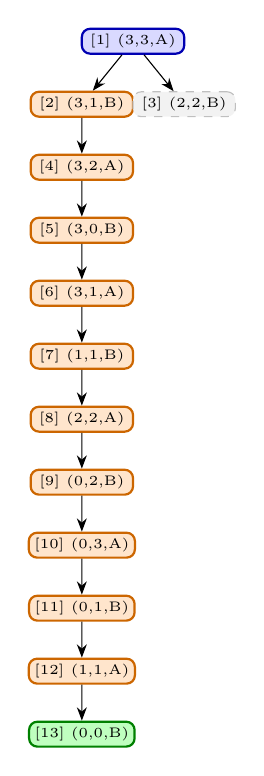
\begin{tikzpicture}[level distance=0.80cm, sibling distance=1.3cm, ->, >=Stealth]
\node[inicio] {[1] (3,3,A)}
  child {node[visitado] {[2] (3,1,B)}
    child {node[visitado] {[4] (3,2,A)}
      child {node[visitado] {[5] (3,0,B)}
        child {node[visitado] {[6] (3,1,A)}
          child {node[visitado] {[7] (1,1,B)}
            child {node[visitado] {[8] (2,2,A)}
              child {node[visitado] {[9] (0,2,B)}
                child {node[visitado] {[10] (0,3,A)}
                  child {node[visitado] {[11] (0,1,B)}
                    child {node[visitado] {[12] (1,1,A)}
                      child {node[meta] {[13] (0,0,B)}}
                    }
                  }
                }
              }
            }
          }
        }
      }
    }
  }
  child {node[novisitado] {[3] (2,2,B)}};
\end{tikzpicture}
\end{minipage}
\hfill
\begin{minipage}[t]{0.48\linewidth}
\centering
\textbf{\scriptsize b) Recorrido por Profundidad (DFS)}\\[4pt]
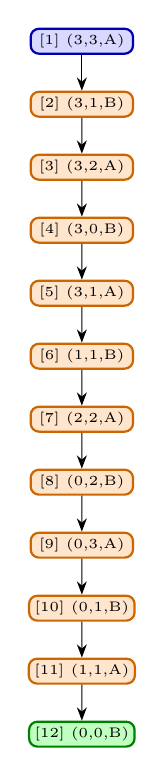
\begin{tikzpicture}[level distance=0.80cm, sibling distance=1.3cm, ->, >=Stealth]
\node[inicio] {[1] (3,3,A)}
  child {node[visitado] {[2] (3,1,B)}
    child {node[visitado] {[3] (3,2,A)}
      child {node[visitado] {[4] (3,0,B)}
        child {node[visitado] {[5] (3,1,A)}
          child {node[visitado] {[6] (1,1,B)}
            child {node[visitado] {[7] (2,2,A)}
              child {node[visitado] {[8] (0,2,B)}
                child {node[visitado] {[9] (0,3,A)}
                  child {node[visitado] {[10] (0,1,B)}
                    child {node[visitado] {[11] (1,1,A)}
                      child {node[meta] {[12] (0,0,B)}}
                    }
                  }
                }
              }
            }
          }
        }
      }
    }
  };
\end{tikzpicture}
\end{minipage}
\caption{Diferenciación gráfica de los recorridos BFS y DFS para Misioneros y Caníbales. Elaboración propia.}
\label{fig:misioneros_bfs_dfs}
\end{figure}

Como muestra la Figura~\ref{fig:misioneros_bfs_dfs}, en el problema de misioneros y caníbales \textbf{BFS (a)} explora las dos opciones iniciales de cruce ($[2]$ con dos caníbales y $[3]$ con un misionero y un caníbal). Al ser $[3]$ un estado sin salida próspera inmediata a corto plazo, el algoritmo lo mantiene generado pero continúa nivel por nivel. Por otro lado, \textbf{DFS (b)} se enfoca exclusivamente en la secuencia lineal de 11 cruces óptimos sin evaluar ramas secundarias muertas, llegando al nodo meta $(0,0,B)$ en menos pasos de exploración global.

\subsection{Análisis Comparativo del Ejercicio 3}

\begin{table}[H]
\centering\small
\renewcommand{\arraystretch}{1.2}
\begin{tabularx}{\linewidth}{@{} l X X @{}}
\toprule
\textbf{Criterio de Evaluación} & \textbf{Búsqueda en Anchura (BFS)} & \textbf{Búsqueda en Profundidad (DFS)} \\
\midrule
\textbf{Nodos Generados} & 16 nodos alcanzables & 16 nodos alcanzables \\
\textbf{Nodos Explorados} & 13 exploraciones & 12 exploraciones \\
\textbf{Profundidad ($d$)} & $d = 11$ cruces & $d = 11$ cruces \\
% \textbf{Uso de Memoria} & $O(b^d)$ — Almacena la frontera por nivel & $O(b \cdot m)$ — Almacena únicamente el camino activo \\
\textbf{Completitud} & Sí & Sí (requiere control estricto de visitados) \\
\textbf{Optimalidad} & Óptimo (garantiza el mínimo de 11 pasos) & No óptimo (en grafos generales puede divergir) \\
\bottomrule
\end{tabularx}
\caption{Análisis de los parámetros de rendimiento para el Ejercicio 3.}
\end{table}

\section{Conclusión}

El desarrollo práctico demuestra de forma clara las diferencias conceptuales y operativas entre los algoritmos de búsqueda sin información:

\begin{itemize}
  \item \textbf{Búsqueda en Anchura (BFS):} Es la estrategia idónea cuando se requiere garantizar la solución más corta (optimalidad en costo uniforme), a costa de un consumo exponencial de memoria en la cola FIFO.
  \item \textbf{Búsqueda en Profundidad (DFS):} Es altamente eficiente en consumo de memoria al operar con una pila LIFO, pero requiere mecanismos rigurosos de detección de ciclos para garantizar completitud y no asegura soluciones óptimas.
\end{itemize}

\referencias
\end{document}